\documentclass[11pt,a4paper]{article}
% Backup to the three-page note jerome-call-2026-10-19.tex (call with Jérôme, 19 October 2026): the email point by
% point, derivations, the full field table, cost, speciation, stress tests, caveats, the 25 September questions.
% Every number is a macro generated from the frozen outputs or a generated table of the paper.
% Shared preamble of jerome-call-2026-10-19.tex (three-page note) and jerome-call-2026-10-19-backup.tex.
% Numbers: macros generated from the frozen outputs (../paper/sections/field-numbers.tex).
\usepackage[T1]{fontenc}
\usepackage[utf8]{inputenc}
\usepackage{lmodern}
\usepackage{amsmath,amssymb}
\usepackage[margin=2.2cm]{geometry}
\usepackage{microtype}
\usepackage{booktabs}
\usepackage{array}
\usepackage{tabularx}
\usepackage{multirow}
\usepackage{graphicx}
\usepackage[font=small,labelfont=bf]{caption}
\usepackage{xcolor}
\usepackage{enumitem}
\usepackage[hyphens]{url}
\usepackage[hidelinks]{hyperref}
\graphicspath{{figures/}{../paper/figures/}}
\setlist{itemsep=0.1em,topsep=0.25em,leftmargin=1.3em}
\setlength{\parindent}{0pt}
\setlength{\parskip}{0.35em}
\renewcommand{\topfraction}{0.9}\renewcommand{\bottomfraction}{0.8}\renewcommand{\textfraction}{0.07}
\renewcommand{\floatpagefraction}{0.85}
\emergencystretch=3em
\newcolumntype{L}{>{\raggedright\arraybackslash}X}
% ===========================================================================
% Shared notation for the internal note and the compendium.
%
% Conventions follow the statistical-physics usage of the diffusion literature
% (Song et al. 2021 for the SDE formulation; Mezard-Montanari 2009 for the
% graphical-model side). Only publicly available sources are cited.
% docs/NOTATION.md is the reference for every symbol below, for the code names
% that carry them, for the collaborators' note, and for the thesis concordance.
%
% Symbol decisions that matter, fixed here once:
%
%   1. K (or K_theta) is the MARKOV TRANSITION KERNEL, everywhere and only.
%      The number of quadrature grid points is N_g. These were previously W and
%      K respectively, which collided; nothing in either document may now use
%      K for a grid size or W for a kernel. The phi^4 transfer operator
%      e^{-W} is \transfer (sans-serif T), never K.
%
%   2. The chain length is L, and every graphical-model statement is indexed by
%      sites. The ambient dimension equals it, n = L, but the two are written
%      separately because they are different concepts and the reader should not
%      have to infer the identification. The number of observed sequences is M,
%      and never the grid size.
%      A translation sentence appears at first use, because much of the
%      diffusion literature uses n for the sample count and d for the dimension.
%
%   3. The decay factor is written e^{-t} in displayed equations. Where a proof
%      abbreviates it, the abbreviation is alpha = e^{-t}, declared, never
%      alpha_t and never anything else (the code's argument `alpha` is the same
%      object).
%
%   4. Gaussian white noise eta is STANDARDISED, <eta(t)eta(t')> = delta(t-t'),
%      so the sqrt(2) is carried explicitly in both the forward and the reverse
%      SDE. This keeps Delta_t = 1 - e^{-2t} consistent throughout.
%
%   5. Vectors are bold lowercase (\vect) and matrices and tensors are bold
%      uppercase (\mat). Scalars, including single sites a_i, stay upright.
%      Anything indexed down to a scalar loses its bold.
%
%   6. BP messages are the cavity messages \lmsg_i, \rmsg_i: both EXCLUDE the
%      local likelihood ell_i, and the site marginal is \lmsg_i ell_i \rmsg_i.
%      (The collaborators' note writes alpha_i = \lmsg_i ell_i and beta_i =
%      \rmsg_i.) Posterior marginals are written out, p(a_i | x), because gamma
%      and xi are taken (6 and 7 below).
%
%   7. The chain's driving noise is eps_i with density p_eps and variance q; the
%      word "innovation" is not used (the 25 Sep call). The linear chain with
%      Laplace driving noise, not "the Laplace AR(1)".
%
%   8. Greek letters with one meaning each: gamma the phi^4 bond variance
%      (the Gaussian reference measure is \gref); xi the correlation length;
%      beta the generalised-Gaussian exponent; delta a misspecification
%      strength; h the lattice spacing (the quadrature spacing is \gridh).
% ===========================================================================

% --- Diffusion -------------------------------------------------------------
\newcommand{\Pz}{P_0}                       % clean distribution
\newcommand{\Pt}{P_t}                       % noised distribution at time t
\newcommand{\Dt}{\Delta_t}                  % 1 - e^{-2t}
\newcommand{\score}{S}                      % S(x,t) = grad log P_t(x)
\newcommand{\gwn}{\vect{\eta}}              % standardised Gaussian white noise (vector)
\newcommand{\tmin}{t_{\min}}
\newcommand{\tmax}{t_{\max}}

% Posterior mean, in bracket notation rather than E[a|x].
\newcommand{\pmean}[1]{\langle #1 \rangle_{x,t}}
\newcommand{\pmeansite}[1]{\langle a_{#1} \rangle_{x,t}}

% --- Vectors and matrices --------------------------------------------------
% Bold lowercase for vectors, bold uppercase for matrices and tensors.
\newcommand{\vect}[1]{\mathbf{#1}}
\newcommand{\mat}[1]{\mathbf{#1}}
\newcommand{\va}{\vect{a}}                  % clean chain, in R^L
\newcommand{\vx}{\vect{x}}                  % noised chain, in R^L
\newcommand{\vz}{\vect{z}}                  % standard normal draw, in R^L
\newcommand{\Sig}{\mat{\Sigma}}             % covariance
\newcommand{\Id}{\mat{I}}                   % identity

% --- Chain and graphical model --------------------------------------------
\newcommand{\nsites}{L}                     % chain length (ambient dimension n = L)
\newcommand{\nseq}{M}                       % number of observed sequences
\newcommand{\ngrid}{N_{\mathrm{g}}}         % number of quadrature grid points
\newcommand{\gridpt}[1]{u_{#1}}             % grid point
\newcommand{\gridh}{\Delta u}                % quadrature grid spacing (h is the lattice spacing)
\newcommand{\halfwidth}{A}                  % grid half-width, domain [-A, A]
\newcommand{\kernel}{K}                     % transition kernel K(a'|a)
\newcommand{\kernelth}{K_{\params}}         % parameterised transition kernel
\newcommand{\like}{\ell_t}                  % unary likelihood factor
\newcommand{\lmsg}{\overrightarrow{m}}      % forward cavity message (excludes ell_i)
\newcommand{\rmsg}{\overleftarrow{m}}       % backward cavity message (excludes ell_i)
\newcommand{\innov}{p_{\varepsilon}}          % driving-noise density
\newcommand{\corr}{\rho}                    % autoregression coefficient
\newcommand{\ivar}{q}                       % driving-noise variance
\newcommand{\ncomp}{C}                      % mixture component count

% --- The phi^4 field (docs/NOTATION.md) ------------------------------------
\newcommand{\Temp}{\Theta}                  % physical temperature (code: T)
\newcommand{\latt}{h}                       % lattice spacing
\newcommand{\bondvar}{\gamma}               % bond variance, gamma = Theta h / s^2
\newcommand{\transfer}{\mathsf{T}}          % transfer operator e^{-W}
\newcommand{\corrlen}{\xi}                  % correlation length (in sites)
\newcommand{\gref}{\mathcal{N}}             % standard Gaussian reference measure (was gamma)

% --- Estimation ------------------------------------------------------------
\newcommand{\params}{\theta}
\newcommand{\Qfun}{\mathcal{Q}}             % EM auxiliary function
\newcommand{\Xis}{\mat{\Xi}}                % expected transition statistic (a matrix)
\newcommand{\Lik}{\mathcal{L}}              % marginal log-likelihood

% --- Operators -------------------------------------------------------------
\newcommand{\E}{\mathbb{E}}
\newcommand{\Prob}{\mathbb{P}}
\newcommand{\Reals}{\mathbb{R}}
\newcommand{\Cov}{\operatorname{Cov}}
\newcommand{\Var}{\operatorname{Var}}
\newcommand{\KL}{D_{\mathrm{KL}}}
\newcommand{\normal}[2]{\mathcal{N}\!\left(#1,#2\right)}
% Gaussian moment projection, defined formally in prop-lmmse: the Gaussian with
% the same first two moments as its (normalised) argument. Named rather than
% written inline because the LMMSE proposition is a statement about WHERE this
% operator is applied, and an unnamed operator cannot carry that.
\newcommand{\Pgauss}{\Pi_{\mathrm{G}}}
\newcommand{\dd}{\,\mathrm{d}}

% --- Estimators ------------------------------------------------------------
\newcommand{\mmse}{\widehat{\va}_{\mathrm{MMSE}}}
\newcommand{\lmmse}{\widehat{\va}_{\mathrm{LMMSE}}}

% --- Pending-data guard -----------------------------------------------------
% Every number in the paper must come from the frozen batch (outputs/frozen/).
% While that batch is running, a slot that still needs a number is marked with
% \needsdata{what}, which renders in loud red with a bracket. It is deliberately
% impossible to miss in a built PDF, so a placeholder cannot be mistaken for a
% result. `tools/check_no_placeholders.sh` greps for it and fails the build if
% any survive.
\providecommand{\needsdata}[1]{{\bfseries\color{red}[PENDING: #1]}}

% --- Repository pointers (shared by the note and the compendium) ------------
% The arrow is drawn only when there IS a second component to point at.
% Four call sites pass an empty second argument to mean "the whole file", and
% those were rendering as "path/to/file.py -> produces the numbers above",
% a dangling arrow running into the prose.
\providecommand{\codepath}[1]{\texttt{\small #1}}
\providecommand{\coderef}[2]{%
  \codepath{#1}\ifx\relax#2\relax\else\,$\rightarrow$\,\texttt{\small #2}\fi}
\providecommand{\codefile}[1]{\texttt{\small #1}}

%% GENERATED by tools/make_paper_numbers.py -- do not hand-edit.
\newcommand{\cmpAnsatzOverGauss}{2{,}272}
\newcommand{\cmpBpMsEightThreads}{0.52}
\newcommand{\cmpBpMsOneFifty}{0.173}
\newcommand{\cmpBpMsOneThread}{0.667}
\newcommand{\cmpCoarseFitSpeedup}{14}
\newcommand{\cmpCoarseLearnedFifty}{1.2\%}
\newcommand{\cmpCoarseOracleHundred}{1.8\times10^{-11}}
\newcommand{\cmpCoarseSpeedupHundred}{6.2}
\newcommand{\cmpCoarseSpeedupOneFifty}{3.9}
\newcommand{\cmpFftCapHi}{1.18}
\newcommand{\cmpFftCapLo}{1.14}
\newcommand{\cmpFftError}{6.7\times10^{-4}}
\newcommand{\cmpFftSlower}{5.8}
\newcommand{\cmpFftSlowerLarge}{2.2}
\newcommand{\cmpFourierAdaptedHi}{47}
\newcommand{\cmpFourierAdaptedLo}{33}
\newcommand{\cmpFourierReach}{\text{53 of 144}}
\newcommand{\cmpGridHi}{151}
\newcommand{\cmpGridLo}{45}
\newcommand{\cmpGruMsOne}{0.063}
\newcommand{\cmpHeadlineAtFifty}{70\%}
\newcommand{\cmpHeadlineAtHundred}{2.2\%}
\newcommand{\cmpHeadlineAtOneFifty}{0.08\%}
\newcommand{\cmpMatmulShareHi}{15.2\%}
\newcommand{\cmpMatmulShareLo}{12.1\%}
\newcommand{\cmpMemMb}{266}
\newcommand{\cmpMemRatioMax}{4.2}
\newcommand{\cmpMemRatioMin}{1.8}
\newcommand{\cmpRatioCpu}{12.5}
\newcommand{\cmpRatioFiftyGru}{2.8}
\newcommand{\cmpRatioGpu}{15.1}
\newcommand{\cmpRatioGpuLarge}{6.2}
\newcommand{\cmpRatioOneGru}{10.6}
\newcommand{\cmpRatioOneTf}{3.2}
\newcommand{\cmpResolvedHundred}{22\%}
\newcommand{\cmpSlopeBatch}{1.03}
\newcommand{\cmpSlopeGrid}{1.16}
\newcommand{\cmpSlopeLength}{1.03}
\newcommand{\cmpTcnMsOne}{0.216}
\newcommand{\cmpTfMsEightThreads}{0.042}
\newcommand{\cmpTfMsOne}{0.208}
\newcommand{\cmpUnetMsOne}{0.152}
\newcommand{\cmpWindowMsOne}{0.023}
\newcommand{\fldBarrierBigM}{32\,768}
\newcommand{\fldBarrierFits}{80}
\newcommand{\fldBarrierOkFits}{78}
\newcommand{\fldBarrierSlope}{0.54}
\newcommand{\fldBimodCold}{0.73}
\newcommand{\fldBimodHot}{0.45}
\newcommand{\fldBpCostLone}{0.51}
\newcommand{\fldBpCostLthree}{2.0}
\newcommand{\fldCleanMixRatioMax}{0.99}
\newcommand{\fldCleanMixRatioMin}{0.90}
\newcommand{\fldCoarseKinkSpread}{11\%}
\newcommand{\fldCorrZMax}{2.86}
\newcommand{\fldDomQuantDevSite}{5.6\%}
\newcommand{\fldDomQuantDevSpline}{10.4\%}
\newcommand{\fldFloorFixedHCold}{0.296}
\newcommand{\fldFloorFixedHHot}{0.184}
\newcommand{\fldInpaintCovMax}{0.893}
\newcommand{\fldInpaintCovMin}{0.890}
\newcommand{\fldInpaintGridCost}{0.01}
\newcommand{\fldInpaintLinErrMax}{4.6\%}
\newcommand{\fldInpaintLinErrMin}{1.5\%}
\newcommand{\fldInpaintLinWidthMax}{9\%}
\newcommand{\fldInpaintLinWidthMin}{7\%}
\newcommand{\fldInpaintOracleCov}{0.89}
\newcommand{\fldInpaintOracleDev}{0.4\%}
\newcommand{\fldInpaintOracleErrMax}{1.0004}
\newcommand{\fldInpaintOracleErrMin}{0.9999}
\newcommand{\fldInpaintOracleWidthMax}{1.004}
\newcommand{\fldInpaintOracleWidthMin}{0.998}
\newcommand{\fldKinkConvergence}{0.04\%}
\newcommand{\fldKinkDevSite}{2.1\%}
\newcommand{\fldKinkDevSpline}{1.1\%}
\newcommand{\fldKinkFit}{0.988}
\newcommand{\fldKinkSlopeCold}{0.87}
\newcommand{\fldKinkSlopeHot}{0.64}
\newcommand{\fldKinkTHigh}{0.29}
\newcommand{\fldKinkTLow}{0.11}
\newcommand{\fldMixDomShortMax}{18\%}
\newcommand{\fldMixDomShortMin}{14\%}
\newcommand{\fldMixFloorMax}{1.021}
\newcommand{\fldMixFloorMin}{1.004}
\newcommand{\fldMixKinkColdMax}{1.42}
\newcommand{\fldMixKinkColdMin}{1.41}
\newcommand{\fldMixSplineBaseA}{9.5}
\newcommand{\fldMixSplineBaseB}{18.2}
\newcommand{\fldNetCostMax}{0.32}
\newcommand{\fldNetCostMin}{0.004}
\newcommand{\fldNetOverSplineMin}{4.1}
\newcommand{\fldNetRatioMax}{24}
\newcommand{\fldNetRatioMin}{14}
\newcommand{\fldOracleGridWorst}{1.3\times10^{-12}}
\newcommand{\fldProjEdgeBase}{0.42}
\newcommand{\fldProjEdgeOthersMin}{0.98}
\newcommand{\fldQuenchEarly}{0.986}
\newcommand{\fldQuenchEq}{0.950}
\newcommand{\fldRawKinkA}{0.120}
\newcommand{\fldRawKinkB}{0.176}
\newcommand{\fldRawKinkC}{0.247}
\newcommand{\fldSiteFloorMax}{0.169}
\newcommand{\fldSiteFloorMin}{0.032}
\newcommand{\fldSiteOverSplineMax}{0.57}
\newcommand{\fldSiteOverSplineMin}{0.41}
\newcommand{\fldSpecCalibDev}{0.003}
\newcommand{\fldSpecExcessCold}{0.47}
\newcommand{\fldSpecExcessHot}{0.07}
\newcommand{\fldSpecNoiseRatioExact}{24}
\newcommand{\fldSpecNoiseRatioTwin}{8.9}
\newcommand{\fldSpecSlope}{0.98}
\newcommand{\fldSpecTcCold}{1.61}
\newcommand{\fldSpecTcHot}{0.46}
\newcommand{\fldSpecTcLfour}{1.03}
\newcommand{\fldSpecTcLonetwentyeight}{1.750}
\newcommand{\fldSpecTcLsixtyfour}{1.72}
\newcommand{\fldSpecTcLtwofiftysix}{1.754}
\newcommand{\fldThetaFits}{96}
\newcommand{\fldThetaOkFits}{96}
\newcommand{\fldTrainEmMax}{5}
\newcommand{\fldTrainEmMin}{8}
\newcommand{\fldTrainNetMax}{38}
\newcommand{\fldTrainNetMin}{9}
\newcommand{\fldWindowFloorHone}{0.55}
\newcommand{\fldWindowFloorHzeroptwofive}{1.20}
\newcommand{\fldWindowRiskHone}{0.149}
\newcommand{\fldWindowRiskHzeroptwofive}{0.118}
\newcommand{\fldWindowSplineHone}{9.2}
\newcommand{\fldWindowSplineHzeroptwofive}{17.6}
\newcommand{\fldXiCold}{19.5}
\newcommand{\fldXiHone}{6.1}
\newcommand{\fldXiHot}{1.06}
\newcommand{\fldXiHzeroptwofive}{22.5}
\newcommand{\genAncestralCostRatio}{731}
\newcommand{\limLapMdn}{0.056}
\newcommand{\limLapMdnAtCap}{5}
\newcommand{\limLapMdnBelowSite}{7}
\newcommand{\limLapMdnBelowUnr}{7}
\newcommand{\limLapSite}{0.103}
\newcommand{\limLapStall}{0.10}
\newcommand{\limLapUnrestricted}{0.068}
\newcommand{\limLapUnrestrictedGain}{1.5}
\newcommand{\limLatentAugFall}{52\%}
\newcommand{\limLatentFirstOverAug}{13.1}
\newcommand{\limLatentFlat}{+0.2\%}
\newcommand{\limLatentFloorRatio}{6.3}
\newcommand{\limLatentWorseMax}{1.71}
\newcommand{\limLatentWorseMin}{1.56}
\newcommand{\limMdnLinearHi}{2.9}
\newcommand{\limMdnLinearLo}{2.1}
\newcommand{\limStrideAgree}{7.6\%}
\newcommand{\limStrideFloor}{0.235}
\newcommand{\limStrideGrowthSite}{25}
\newcommand{\limStrideGrowthSpline}{14}
\newcommand{\limStrideMdnAtCap}{11}
\newcommand{\limStrideMdnBelow}{16}
\newcommand{\limStrideMdnRatio}{0.40}
\newcommand{\limStrideOneRatio}{3.0}
\newcommand{\limStrideSiteRisk}{0.040}
\newcommand{\limStrideSplineRisk}{0.036}
\newcommand{\limSymGainMax}{39\%}
\newcommand{\limSymGainMin}{32\%}
\newcommand{\limUnrestrictedGrowthA}{2.8}
\newcommand{\limUnrestrictedGrowthB}{5.5}
\newcommand{\limUnrestrictedPriceMax}{5.5}
\newcommand{\limUnrestrictedPriceMin}{2.5}
\newcommand{\lvlCrossA}{0.98}
\newcommand{\lvlCrossB}{2.07}
\newcommand{\lvlFirstLevelsA}{8}
\newcommand{\lvlFirstLevelsB}{10}

\newcommand{\fals}[1]{\emph{#1}}

\renewcommand{\thesection}{B\arabic{section}}

\title{\textbf{Backup: the $\phi^4$ field and the 25 September questions}}
\author{Giovanni Mantovani}
\date{Call with Jérôme, 19 October 2026}

\begin{document}
\maketitle
\vspace{-1.5em}
\section{Your email, point by point}
\label{app:email}

\begin{table}[h]
\centering\small
\caption{Your email, point by point.}
\label{tab:email}
\begin{tabularx}{\textwidth}{@{}>{\raggedright\arraybackslash}p{0.30\textwidth}L@{}}
\toprule
Your point & What we did, and what came out \\
\midrule
Snapshots are exactly Markov; grid BP is an exact reference & Yes. The oracle on the 401-point grid agrees with a four
times finer grid to $\fldOracleGridWorst$ on every cell. \\
The mixture-of-noise family is misspecified; a learned kernel is needed & Confirmed: the mixture sits on the Gaussian closure,
$\fldMixFloorMin$--$\fldMixFloorMax$ times it. \\
Parametrise a pair energy $W_\params$; Boltzmann learning; the E-step is the Fisher identity & Done, with five parameters
(main note, Section~2); best arm everywhere. One addition: the directed kernel and the symmetric pair energy are the
same model class (every such kernel is reversible, \ref{app:model}). \\
Gaussian closure should fail badly & It fails, and more than expected: moment-projected BP is not even well-posed here
(\ref{app:model}). The Gaussian answer is the linear floor: $0.27$ on the base cell against $0.03$ for the site energy. \\
Choose $\latt$ near the correlation length, or treat $\latt$ as a parameter & Two axes: a temperature sweep at fixed
correlation length ($\corrlen\approx6$ sites), and a refinement $\latt=1,\tfrac12,\tfrac14$ at fixed physical length; plus a
fixed-$\latt$ sweep for the physics. \\
Fixed-window networks lose under refinement; BP does not care & Confirmed (\ref{app:cost}). \\
Domain length grows like $e^{\Delta E/\Temp}$; no transition in 1D & Smooth crossover, $\corrlen$ from $\fldXiHot$ to $\fldXiCold$
sites as $\Temp$ goes from $2$ to $0.2$. \fals{The fitted kink energy is $\fldKinkFit$, not $2\sqrt2/3\approx0.943$}: these
temperatures are not cold enough. \\
Use the temperature sweep to study speciation & Done (main note, Figure~3; \ref{app:speciation}). \\
Exact sampling, no equilibration issues & Data are exact steps of the true kernel (rejection from the tilted walk), the first
site after a burn-in that forgets the start to $10^{-12}$; an inverse-CDF sampler on the transfer matrix agrees. \\
Optimise grid BP; Fourier not so promising & Agreed. The cheap lever is a coarser grid: on $101$ points the $\phi^4$ kernels lose
nothing and BP is $\cmpCoarseSpeedupHundred$ times faster than on $401$. \\
Frame the theory neutrally, with the linear chain as a first example & Drafted this way (general Markov kernel; linear chain first,
field second); to be cut down. \\
\bottomrule
\end{tabularx}
\end{table}

\section{The model and the estimator in more detail}
\label{app:model}

\textbf{Directed or symmetric? The same class.} Any tilted walk $\kernel_g(a'\mid a)=\normal{a';a}{\bondvar}\,g(a')/Z_g(a)$ is
reversible, with invariant law $\pi_g\propto g\,Z_g$, because $\pi_g(a)\kernel_g(a'\mid a)\propto g(a)\,g(a')\,\normal{a';a}{\bondvar}$
is symmetric. It is the Gibbs chain of the pair energy $W(a,a')=(a'-a)^2/2\bondvar+f(a)+f(a')$ with $f=-\tfrac12\log(g/Z_g)$. So the choice is only about
parametrisation: a flexible tilt $\log g$ (a spline, $25$ numbers, or a Legendre polynomial, $7$) or the site energy itself ($5$,
a quartic for the field).

\textbf{Fitting.} The E-step accumulates the expected pair counts $\Xis(a,a')$ from BP; the M-step increases
$\Qfun(\params)=\langle\Xis,\log\kernelth\rangle$ by L-BFGS, with the gradient through the perturbation theory of the Perron vector
(one eigensolve per evaluation; not concave, so generalised EM). The stopping point is chosen on a validation set (\ref{app:honest}).

\textbf{What the Gaussian closure is here.} Forcing the messages to be Gaussian (moment projection, which on a linear chain is
exactly the Kalman smoother) is not a usable estimator on the field: far from the bulk the kernel jumps back towards it almost
regardless of where it starts, so the backward messages are nearly flat across the grid and their projection discards them
($\fldProjEdgeBase$ of a projected message's mass in the outer $5\%$ of the grid on the base cell, $\fldProjEdgeOthersMin$ or more
on the others). The Gaussian arm is therefore the covariance twin's exact answer, the best linear estimator, in closed form.

\textbf{The cells.} The three hotter cells keep the correlation length at about six sites by solving for $\latt$, matching the
linear-chain laboratory at second order; the refinements keep the physical length fixed. The floor column is how much there is
to gain beyond a Gaussian model.

%% GENERATED by tools/make_paper_numbers.py -- do not hand-edit.
\begin{table}[t]
\setlength{\tabcolsep}{4pt}
\centering
\small
\caption{The six cells of the field laboratory: temperature $\Temp$, lattice spacing $\latt$ (solved on the three hotter cells to hold the correlation length fixed), chain length $\nsites$, correlation length $\corrlen$ in sites, excess kurtosis of the marginal (kurt.), and the schedule-pooled relative score error of the best linear estimator (floor) and of the isotropic score (iso.), mean of two replicates.}
\label{tab:fieldcells}
\begin{tabular}{@{}rrrrrrr@{}}
\toprule
$\Temp$ & $\latt$ & $\nsites$ & $\corrlen$ & kurt. & floor & iso. \\
\midrule
0.3 & 1.000 & 32 & 6.1 & $-1.35$ & 0.269 & 0.674 \\
0.5 & 0.419 & 32 & 6.2 & $-0.88$ & 0.115 & 0.657 \\
1.0 & 0.226 & 32 & 6.2 & $-0.59$ & 0.058 & 0.657 \\
2.0 & 0.150 & 32 & 6.2 & $-0.46$ & 0.041 & 0.656 \\
0.3 & 0.500 & 64 & 11.5 & $-1.25$ & 0.162 & 0.714 \\
0.3 & 0.250 & 128 & 22.5 & $-1.22$ & 0.098 & 0.750 \\
\bottomrule
\end{tabular}
\end{table}


\section{More on the results}
\label{app:results}

%% GENERATED by tools/make_paper_numbers.py -- do not hand-edit.
\begin{table*}[t]
\setlength{\tabcolsep}{6pt}
\centering
\footnotesize
\caption{Risk divided by the linear floor (a Gaussian closure scores $1$), mean over sixteen seeds, of every estimator on the six cells; the first four columns are the temperature sweep at matched correlation length, the last two refine the base cell at fixed physical length. EM's stopping point and each network's checkpoint are selected by the held-out risk against the exact score. A superscript counts failed fits, excluded from the mean; a dash means all sixteen failed. Bold: smallest in its column.}
\label{tab:fieldscore}
\begin{tabular}{@{}rlrrrrrr@{}}
\toprule
$\nseq$ & estimator & $\Temp=0.3$ & $0.5$ & $1$ & $2$ & $\latt=0.5$ & $\latt=0.25$ \\
\midrule
128 & site energy (5) & \textbf{0.139} & \textbf{0.269} & \textbf{0.534} & \textbf{0.630} & \textbf{0.136} & \textbf{0.130} \\
 & spline tilt (25) & 0.218 & 0.454 & 1.111 & 1.478 & 0.231 & 0.235 \\
 & Legendre tilt (7) & 0.394 & 0.354 & 0.647 & 0.816 & 0.330 & 0.387$^{6}$ \\
 & MDN & 0.468 & 0.900 & 1.724 & 2.457 & 0.476 & 0.585 \\
 & mixture (paper) & 1.018 & 1.039 & 1.187 & 1.279 & 1.016 & 1.017 \\
 & window, ISM & 1.026 & 4.396 & 6.264 & 8.735 & 1.495 & 2.237 \\
 & transformer, ISM & 3.284 & 9.752 & 8.509 & 14.487 & 3.591 & 4.729 \\
 & window, DSM & 0.829 & 2.339 & 4.149 & 5.786 & 1.125 & 1.580 \\
 & transformer, DSM & 1.787 & 4.359 & 8.034 & 11.571 & 1.887 & 2.129 \\
\midrule
2048 & site energy (5) & \textbf{0.033} & \textbf{0.072} & \textbf{0.141} & \textbf{0.169} & \textbf{0.040} & \textbf{0.032} \\
 & spline tilt (25) & 0.060 & 0.134 & 0.280 & 0.429 & 0.073 & 0.068 \\
 & Legendre tilt (7) & 0.074 & 0.092 & 0.165 & 0.243 & 0.111 & -- \\
 & MDN & 0.228 & 0.422 & 0.737 & 0.837 & 0.310 & 0.420 \\
 & mixture (paper) & 1.004 & 1.004 & 1.014 & 1.021 & 1.010 & 1.016 \\
 & window, ISM & 0.552 & 1.284 & 2.457 & 3.559 & 0.776 & 1.196 \\
 & transformer, ISM & 1.354 & 2.706 & 2.440 & 3.237 & 1.368 & 1.020 \\
 & window, DSM & 0.484 & 1.174 & 2.287 & 3.334 & 0.701 & 1.030 \\
 & transformer, DSM & 0.533 & 1.225 & 2.156 & 3.043 & 0.622 & 0.780 \\
\bottomrule
\end{tabular}
\end{table*}


\begin{figure}[t]
\centering
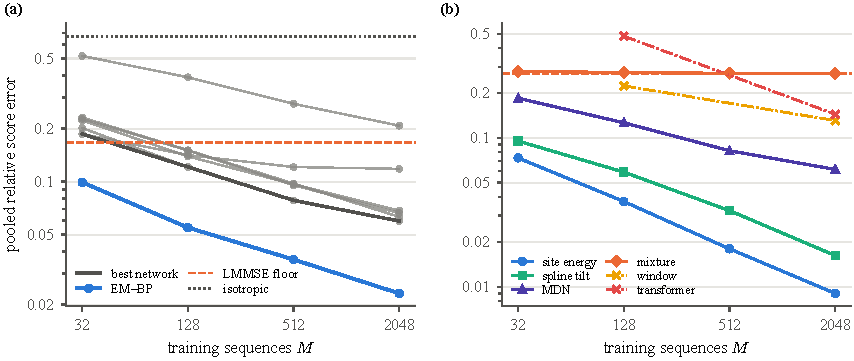
\includegraphics[width=\textwidth]{ff-sample-efficiency.pdf}
\caption{Pooled error against the number of training sequences. (a) The paper's linear chain with Laplace driving noise: EM--BP
with the 25-number mixture kernel against the best network (trained on clean sequences; the other architectures in grey), the
LMMSE floor and the isotropic score. (b) The $\phi^4$ base cell ($\Temp=0.3$, $\latt=1$): the site energy improves steadily, the
paper's mixture stays on the dashed linear floor, the networks (DSM) start above it.}
\label{fig:efficiency}
\end{figure}

\begin{itemize}
\item With $\nseq=128$ (Table~\ref{tab:fieldscore}) the site energy is again best on every cell, and every network is above the
floor on every cell with $\Temp\ge0.5$.
\item \fals{We had predicted the site energy would be within $10\%$ of the spline; it is about twice as good.} The right five
parameters beat a flexible 25.
\item The mixture's samples show its failure: $\fldMixKinkColdMin$--$\fldMixKinkColdMax$ times too many kinks on the cold cells and
domains $\fldMixDomShortMin$--$\fldMixDomShortMax$ too short at the median, while the site energy's samples are within
$\fldKinkDevSite$ in kink density and $\fldDomQuantDevSite$ at every domain-length quantile, indistinguishable from exact samples.
\item The networks are at least $\fldNetOverSplineMin$ times the spline's error, and above the linear floor on every cell with
$\Temp\ge0.5$, whichever training recipe; they do beat the mixture on the cold cells. The MDN kernel is below the floor at
$\nseq=2048$ on every cell, but well above the tilts.
\item Physics: on the base cell $\hat\Temp/\Temp=1.000\pm0.023$ and barrier $0.247\pm0.011$ against $0.25$ (mean $\pm$ s.d.\ over
sixteen seeds, $\nseq=2048$). At $\Temp=2$ the barrier is learned slowly: its error falls like $\nseq^{-\fldBarrierSlope}$ and all
sixteen seeds are within $20\%$ at $\nseq=\fldBarrierBigM$, a sample-size limit, not a floor. The 25-number spline does not pin the
potential down at $\Temp=2$ (main note, Figure~2b).
\end{itemize}

\section{Refinement and cost}
\label{app:cost}

\textbf{Refinement.} The correlation length in sites grows like $1/\latt$ ($\fldXiHone$ to $\fldXiHzeroptwofive$ from $\latt=1$ to
$\tfrac14$). The window CNN's radius was screened on each lattice and the screen picked $2$, $4$, $8$ sites, a constant
physical reach ($8$ was the largest offered). Trained on noisy copies (ISM) with $\nseq=2048$, its absolute error falls
($\fldWindowRiskHone\to\fldWindowRiskHzeroptwofive$), but relative to the spline it grows from $\fldWindowSplineHone$ to
$\fldWindowSplineHzeroptwofive$, and relative to the floor from $\fldWindowFloorHone$ to $\fldWindowFloorHzeroptwofive$: on the
finest lattice the window is worse than the Gaussian closure. Per step the field becomes nearly Gaussian as $\latt\to0$ (your
$O(\latt)$ caveat), the floor falls ($0.269\to0.098$), and the site energy still stays at $3$--$4\%$ of it: the structure builds up
over many sites, and BP collects it. Whether a wider window closes the gap was not tested.

\begin{figure}[t]
\centering
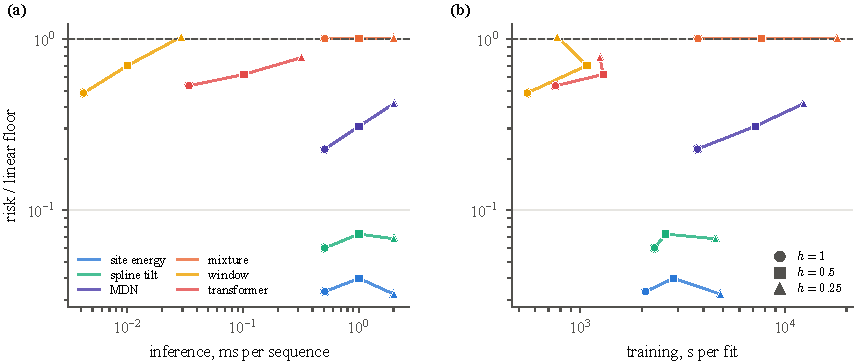
\includegraphics[width=\textwidth]{fig-field-runtime.pdf}
\caption{Error over the linear floor against (a) inference time per sequence and (b) training time per fit, at $\Temp=0.3$ on
$\latt=1,\tfrac12,\tfrac14$ (circle, square, triangle; $32$, $64$, $128$ sites), $\nseq=2048$. Inference: eight threads, batch
512, the largest network variants. Training: shared nodes, indicative only. BP's time is the same for every kernel.}
\label{fig:runtime}
\end{figure}

\textbf{Cost.} Figure~\ref{fig:runtime}: the networks own the cheap end ($\fldNetCostMin$--$\fldNetCostMax$\,ms per sequence) and
the structured kernels the accurate end ($\fldBpCostLone$--$\fldBpCostLthree$\,ms for BP), with nothing in between. The grid is
the lever. With the true $\phi^4$ kernel, BP on $101$ points is exact to $\cmpCoarseOracleHundred$; the learned site energy and
spline refitted on $101$ points have the same error as on $401$ to three digits (at most $\cmpCoarseLearnedFifty$ off at $51$),
the EM fit is about $\cmpCoarseFitSpeedup$ times faster, and on one thread BP takes $0.107$\,ms per sequence at $101$ points
against $\cmpBpMsOneThread$\,ms at $401$. The paper's mixtures need about $151$ points, because with much data they learn
components narrower than a $101$-point spacing.

\section{Speciation in detail}
\label{app:speciation}

For a noisy snapshot the exact posterior gives each site $p_i=P(a_i>0\mid\vx)$; the commitment $|2p_i-1|$ goes from $0$ (both
wells equally likely) to $1$ (the site has chosen), and $t_c$ is the level where its site average crosses $\tfrac12$. All five
registered predictions on commitment held:
\begin{itemize}
\item the posterior is calibrated: the share of signs guessed right equals $(1+\text{commitment})/2$ to $\fldSpecCalibDev$;
\item colder fields commit earlier in the reverse process: $t_c$ falls from $\fldSpecTcCold$ at $\Temp=0.2$ to $\fldSpecTcHot$ at
$\Temp=2$;
\item the exact posterior commits before its Gaussian twin at every temperature, by $\fldSpecExcessCold$ in $t$ when coldest
and $\fldSpecExcessHot$ when hottest. At $\Temp=0.2$ it is half-committed when the noise variance is $\fldSpecNoiseRatioExact$ times
the signal's, the twin only at $\fldSpecNoiseRatioTwin$: the two humps, not just the correlations, decide when it commits;
\item $t_c$ grows with the chain length ($\fldSpecTcLfour$ at $\nsites=4$, $\fldSpecTcLsixtyfour$ at $64$) and stops once the
chain is several domains long ($\fldSpecTcLonetwentyeight$, $\fldSpecTcLtwofiftysix$ at $128$, $256$);
\item below the correlation length, $t_c$ moves one-for-one with $\tfrac12\ln(1+\lambda_{\max})$ (slope $\fldSpecSlope$),
$\lambda_{\max}$ the largest covariance eigenvalue: the finite-chain analogue of the speciation time $\tfrac12\ln\lambda_{\max}$ of
Biroli, Bonnaire, de~Bortoli and Mézard.
\end{itemize}
\fals{The dilute-kink law $\corrlen\propto\Temp^{1/2}e^{E_{\mathrm{kink}}/\Temp}$, fitted on $\Temp\in[0.1,0.3]$, returns a barrier
of $\fldKinkFit$ against $2\sqrt2/3$ (predicted within $2\%$).} The local slope approaches the theory as $\Temp$ falls, so the
law looks right but these temperatures do not pin its constant; the lattice itself is converged ($\corrlen$ moves by
$\fldKinkConvergence$ from $\latt=1/16$ to $1/32$).

\section{Where it stops working, and where a neural kernel pays}
\label{app:limits}

\begin{table}[h]
\centering\small
\caption{Stress tests. ``Floor'' is the best linear estimator. Sixteen seeds unless stated.}
\label{tab:limits}
\begin{tabularx}{\textwidth}{@{}>{\raggedright\arraybackslash}p{0.27\textwidth}L@{}}
\toprule
Test & Outcome \\
\midrule
Observe every 4th site (clean fits; the kernel is $\kernel^4$, no longer a tilted walk) & Site energy and spline worsen
$\limStrideGrowthSite\times$ and $\limStrideGrowthSpline\times$ but stay far below the floor ($\limStrideSiteRisk$, $\limStrideSplineRisk$
against $\limStrideFloor$). The MDN is below the site energy in $\limStrideMdnBelow$ of 16 seeds, at $\limStrideMdnRatio$ times its
error; at stride 1 the site energy is $\limStrideOneRatio$ times better than the MDN. \\
A chain outside the class: a Laplace bond $|a'-a|$ on a double well (noisy fits, 8 seeds) & At $\nseq=2048$ the site energy
stalls at $\limLapSite$; a 100-number unrestricted kernel reaches $\limLapUnrestricted$, the MDN $\limLapMdn$ (below the site
energy in $\limLapMdnBelowSite$ of 8 seeds). \\
The 100-number unrestricted kernel on the true field & Costs $\limUnrestrictedPriceMin$--$\limUnrestrictedPriceMax$ times the site
energy. \fals{The price grows with $\nseq$; we predicted it would shrink.} Useful as a misspecification test, not as the
estimator. \\
A hidden sign shared by the whole sequence (Gaussian test chain; the data are not Markov) & A first-order kernel stalls
($\limLatentFlat$ from 4 times more data) at $\limLatentWorseMin$--$\limLatentWorseMax$ times the floor. BP on the augmented state
(value, sign) repairs it: $\limLatentFloorRatio$ times below the floor. \\
Snapshots after a quench (not Gibbs; reference is the clean snapshot) & The site energy beats an empirical Gaussian smoother at
every time (ratio $\fldQuenchEarly$ early, $\fldQuenchEq$ at equilibrium); the spline adds nothing. \\
Missing data: hide sites, sample posteriors by FFBS & The learned site energy matches the oracle within $\fldInpaintOracleDev$ in
error and interval width, coverage $\fldInpaintCovMin$--$\fldInpaintCovMax$ for a nominal $0.90$. On the cold cell a Gaussian
smoother is only $\fldInpaintLinErrMin$--$\fldInpaintLinErrMax$ worse, with $\fldInpaintLinWidthMin$--$\fldInpaintLinWidthMax$
wider intervals. \\
\bottomrule
\end{tabularx}
\end{table}

In short (Table~\ref{tab:limits}), a neural kernel earns its parameters when the simple family is wrong (stride 4; the Laplace bond), by $1.8$--$2.5$ times
against the best Gaussian-bond kernel, and not when it is right. On the paper's chain it loses to the 25-number mixture in
64 of 64 comparisons. In both winning cases the MDN was still improving when its budget ended (11 of 16 and 5 of 8 fits), so its
numbers there are upper bounds.

\section{What we do not claim}
\label{app:honest}

\begin{itemize}
\item \textbf{Speed.} BP is slower per sequence than a network. On the 401-point grid with eight threads it is
$\cmpRatioCpu\times$ the transformer on CPU and $\cmpRatioGpu\times$ on an H200. On one thread the gap narrows ($3.2\times$ at
$401$ points) and at $101$ points BP is faster than the transformer, but still slower than the GRU. The networks timed are the
largest screened variants.
\item \textbf{Stopping rule.} Every arm's stopping point or checkpoint, networks included, is picked with the exact score on a
validation set. With an oracle-free rule for EM (held-out likelihood) the site energy is at $4$--$23\%$ of the floor instead of
$3$--$17\%$.
\item \textbf{Small data.} With $\nseq=32$ on the two hottest cells the site energy is above the floor ($1.37$, $1.43$); it wins on
average from $\nseq=128$, and in 16 of 16 seeds from $\nseq=512$.
\item \textbf{Failed predictions,} beyond those above: \fals{at $\nseq=128$, $\Temp=2$ the mixture beats the spline in 12 of 16 seeds;
the 7-number Legendre tilt crashes on the finest lattice (39 failed fits); the barrier at $\Temp=1$ is within $20\%$ in 14 of 16
seeds, not 16; the information-decay theorem's $e^{-8t}$ regime is not reached by $t=3$ (ratio $0.73$--$0.94$, unresolved);
the raw count of sign changes is not a lattice-independent kink density (we count kinks after merging short runs).}
\item \textbf{Unexplained:} why the unrestricted kernel's price over the site energy grows with data.
\end{itemize}

\section{The 25 September questions}
\label{app:questions}

Answered in the order of the call. The linear chain is $a_{i+1}=\corr a_i+\varepsilon_i$, $\corr=0.85$, Laplace driving noise,
$\nsites=32$, unless stated.

\textbf{Q1. Gaussian messages = Gaussian score = Kalman?} Yes. On a linear chain, BP whose messages are projected onto Gaussians
returns exactly the best linear estimator of the covariance-matched Gaussian chain,
$\lmmse(\vx)=e^{-t}\Sig(e^{-2t}\Sig+\Dt\Id)^{-1}\vx$, which is the Rauch--Tung--Striebel smoother. The hypothesis that matters is
that the first message is Gaussian (or projected) too; without it the claim is false, by $4\times10^{-2}$ at the first site in a
computed counterexample. Check: grid BP, the closed form and an independent RTS smoother agree to $1.9\times10^{-13}$.
\fals{Projected BP run on the same 401-point grid is off by up to $0.26$: its backward messages widen past the grid's edge.} Not
new: the thesis had it; the paper now says ``Kalman''.

\textbf{Q2--Q4. Do messages stay in a finite family?} Your family, a Gaussian pushed once through the chain,
$\normal{m}{v}$ dilated by $\corr$ and convolved with $\innov$, is exact at the first site and very close afterwards:
$\cmpAnsatzOverGauss\times$ smaller KL than a plain Gaussian and $78\times$ smaller than a 4-parameter Gaussian+Laplace at low
noise. But it is not closed, $(G*\innov)\cdot\mathcal N\neq G'*\innov$: the interior error is above the quadrature floor in 432 of
432 configurations, and does not move when the grid is doubled. The Gaussian closes; we have no proof about other families.
\fals{We predicted the family would do best at high noise; it does worst there,} because with a flat likelihood the recursion
drives messages to the stationary law, an infinite convolution.

\textbf{Q5. Fourier BP?} Two of the three operations are free in Fourier space, which gives the message in closed form,
$\varphi_{k+1}(\omega)=\varphi_\mu(\corr^k\omega)\prod_{j<k}\varphi_\varepsilon(\corr^j\omega)$ (checked against grid BP to
$2\times10^{-8}$). The likelihood is the hard step, a convolution in $\omega$ of width $e^{-t}/\sqrt{\Dt}$, widest at low noise.
As a representation, Fourier modes on a window adapted to each message need $\cmpFourierAdaptedLo$ numbers (KL $10^{-2}$) or
$\cmpFourierAdaptedHi$ ($10^{-4}$) against the grid's $\cmpGridLo$ and $\cmpGridHi$, close to your ``20 modes''; but they reach
$10^{-4}$ in only \cmpFourierReach{} cases and adding modes can make it worse, so a solver cannot choose a truncation. Cumulant
(Gram--Charlier) truncation does not converge: Cramér's condition fails for every message, and adding cumulants makes the
reconstruction worse in 144 of 144 cases. And the transition step is only $\cmpMatmulShareLo$--$\cmpMatmulShareHi$ of a sweep, so
making it free buys at most $\cmpFftCapLo$--$\cmpFftCapHi\times$; our FFT version is $\cmpFftSlower\times$ slower at $401$ points.
The coarse grid is the better trick (\ref{app:cost}).

\textbf{Q6. A neural network for the kernel?} It trains through BP and loses where a small kernel is right: on the linear chain
the 1{,}516-parameter MDN is worse than the 25-number mixture in 64 of 64 comparisons ($\limMdnLinearLo$--$\limMdnLinearHi\times$)
and worse than the best plain score network. \fals{We predicted it would sit between the two.} It wins where the simple family is
wrong (\ref{app:limits}). This is the overfitting you predicted in the call.

\textbf{Q7. Time per posterior mean?} See \ref{app:honest}: BP is slower ($\cmpBpMsEightThreads$ against
$\cmpTfMsEightThreads$\,ms, eight threads; on the H200 $15\times$ at batch 512, $6\times$ at 2048, because BP is latency-bound).
What scales well is training: the EM M-step costs the same whatever $\nseq$ (the E-step is linear in $\nseq$), because the kernel
is evaluated on the grid only.

\textbf{Q8. Generation without a score?} Yes. On a chain, sampling site by site from the kernel is exact, and it is
$\genAncestralCostRatio\times$ cheaper than a 200-step reverse SDE at equal error (eight threads, 2{,}048 sequences). A Gaussian
score generates Gaussian samples (excess kurtosis of $a_{i+1}-0.85a_i$ about $0$ against $1.92$).

\textbf{Q9. Fixed $t$ or pooled?} Per level: EM--BP beats every network at all twelve levels, and beats the Gaussian oracle at
the $\lvlFirstLevelsA$ ($\nseq=128$) or $\lvlFirstLevelsB$ ($\nseq=2048$) lowest. Above that the non-Gaussian structure left is
smaller than the kernel's estimation error; the crossover moves from $t\approx1$ to $t\approx2$ with 16 times more data.
\fals{We predicted first place at every level.}

\textbf{Q10. Information about $\corr,\beta$ or about $\kappa_2,\kappa_4$?} Recomputed, not relabelled. With $\kappa_2=q$,
$\kappa_4=\gamma_2(\beta)q^2$ and $J=\partial(\corr,\kappa_2,\kappa_4)/\partial(\corr,q,\beta)$, the efficiency of coordinate $k$ is
$1/(j_k^\top I_\params^{-1}j_k)$; a relabel would be wrong by $1.6$--$1526\times$. The message survives: fourth-order information
falls about $700\times$ more than second order from $t=0.05$ to $t=3$. Following your advice it is a supporting result, not
the headline.

\textbf{Q11. Scaling in $\nseq$ and $\nsites$?} The call's answer was wrong. A sweep is $O(\nsites\,\ngrid^2 B)$ operations for $B$
sequences: measured slopes $\cmpSlopeBatch$ in $B$, $\cmpSlopeLength$ in $\nsites$, and $\cmpSlopeGrid$ (not $2$) in $\ngrid$,
because element-wise work and memory traffic dominate the matrix product. Memory: about $\cmpMemMb$\,MB for 512 sequences of 32
sites, $\cmpMemRatioMin$--$\cmpMemRatioMax$ times the largest network.

\textbf{Your other requests.} Figures first, with a summary figure: done (the draft opens with one). Labels of the information
plot: re-plotted in cumulant coordinates. Notation: one table; ``driving noise'' instead of ``innovation'', ``linear chain''
instead of AR(1). Clean-input network arm: dropped.

\section{To discuss}
\label{app:discuss}
\begin{enumerate}[leftmargin=1.6em]
\item \textbf{Is this enough for a paper,} as you suggested: the general Markov kernel, the linear chain as the first example
and the $\phi^4$ field as the second? Venue and timeline.
\item \textbf{What to cut.} The draft is far over an 8-page body. Which five or six figures carry it?
\item \textbf{The headline.} ``Learn the local law, infer globally; the kernel family is the modelling choice'', with the
neural kernel as the test of when flexibility pays?
\item \textbf{Marc.} How to involve him from here.
\item \textbf{The defence.} Can I show the field results as further work on Friday?
\end{enumerate}

\vfill
{\footnotesize\raggedright Sources: registry files \path{experiments/registry/E*.json} and the frozen outputs they list (field: E32--E34,
E36--E37, E41--E50; questions: E22--E31, E39--E40, E47); full detail in \path{reports/field-laboratory-2026-10-01.pdf} and
\path{docs/JEROME_CALL_2026-09-25.md}.\par}

\end{document}
